\documentclass [a4paper] {article}

\usepackage[spanish]{babel} 
\usepackage[utf8]{inputenc} 
\usepackage{multirow} 
\usepackage{float} 

\title{R-PL3}
\author{Gabriel López, Sergio Sanz, Álvaro Zamorano}

\usepackage{Sweave}
\begin{document}
\Sconcordance{concordance:G16-p3.tex:G16-p3.Rnw:%
1 10 1 1 0 12 1 1 2 1 0 1 1 3 0 1 2 2 1 1 2 1 0 1 1 3 0 1 2 35 1 1 2 4 0 1 2 3 1 1 2 4 0 1 2 4 1 1 2 1 0 1 1 15 0 1 2 3 1 1 2 1 0 1 1 3 0 1 2 1 1 1 2 %
1 0 1 1 13 0 1 2 2 1 1 2 4 0 1 2 4 1 1 2 1 0 1 1 13 0 2 2 1 0 1 1 3 0 1 2 23 1 1 2 1 0 1 1 3 0 1 2 5 1 1 2 1 0 1 1 11 0 1 2 6 1 1 2 1 0 2 1 3 0 1 2 3 %
1 1 2 1 0 1 1 3 0 1 2 33 1 1 2 1 0 1 1 3 0 1 2 3 1 1 2 1 0 1 1 17 0 1 2 2 1 1 2 4 0 1 2 3 1 1 2 1 0 1 1 21 0 2 2 4 0 1 2 8 1 1 2 1 0 1 1 3 0 1 2 2 1 %
1 2 11 0 1 1 10 0 1 1 10 0 1 1 11 0 1 2 6 1 1 2 1 0 1 1 25 0 1 2 2 1 1 2 4 0 1 2 8 1 1 2 1 0 2 1 3 0 1 2 29 1 1 2 1 0 1 1 15 0 1 2 2 1 1 2 4 0 1 2 17 %
1 1 2 1 0 5 1 3 0 1 2 2 1 1 2 1 0 1 1 3 0 1 2 2 1 1 2 1 0 1 1 3 0 1 2 3 1 1 2 1 0 1 1 3 0 1 2 2 1 1 2 1 0 1 1 3 0 1 2 7 1 1 2 1 0 1 1 3 0 1 2 2 1 1 2 %
1 0 1 1 3 0 1 2 3 1 1 2 1 0 1 1 14 0 1 1 12 0 1 1 12 0 1 1 12 0 1 1 15 0 1 1 15 0 1 1 10 0 1 2 2 1 1 2 6 0 1 1 6 0 1 2 8 1 1 2 11 0 1 2 2 1 1 2 4 0 1 %
2 4 1 1 2 7 0 1 2 6 1 1 2 1 0 1 1 5 0 1 2 9 0 1 1 6 0 1 2 3 1}


\maketitle

\graphicspath{ {./tmp/} }

\section{Ejercicio realizado en clase.}
Para obtener la \textbf{función de clasificación} mediante el algoritmo construcción
de \textbf{árboles de decisión de Hunt} es necesario usar los paquetes \texttt{rpart} y
\texttt{tree}. Estos paquetes hay que descargarlos desde la página de CRAN y para instalarlos
hay que ejecutar el siguiente código:

\begin{Schunk}
\begin{Sinput}
> install.packages("./Paquetes/rpart_4.1-15.zip")
> install.packages("./Paquetes/tree_1.0-40.zip")
\end{Sinput}
\end{Schunk}

\bigskip
De esta forma, los paquete únicamente estarán instalados. Para poder usarlos es necesario cargarlos:
\begin{Schunk}
\begin{Sinput}
> library(rpart)
> library(tree)
\end{Sinput}
\end{Schunk}

\begin{itemize}
\item Con rpart obtendremos las particiones recursivas para la clasificación y los árboles de decisión.
\item Con tree, los árboles de clasificación y regresión.
\end{itemize}

%%%%%%%%%%%%%%%%%%%%%%%%%%%%%%%%%%%%%%%%%%%%%%%%%%% 1.1 %%%%%%%%%%%%%%%%%%%%%%%%%%%%%%%%%%%%%%%%%%%%%%%%%%%

\subsection{Función de clasificación.}
Los datos a usar en este primer ejercicio se componen de 9 calificaciones de estudiantes compuestas por
Teoría, Laboratorio, Prácticas y Calificación Global.

\bigskip
Para introducir estos datos en el algoritmo a usar es necesario tener un fichero \texttt{.txt} con el
siguiente aspecto.
\begin{table}[H]
\begin{center}
\begin{tabular}{|c|c|c|c|c|}
\hline
Suceso & Teoría & Lab & Prac & Calif\\
\hline \hline
s1 & A & A & B & Ap \\ \hline
s2 & A & B & D & Ss \\ \hline
s3 & D & D & C & Ss \\ \hline
s4 & D & D & A & Ss \\ \hline
s5 & B & C & B & Ss \\ \hline
s6 & C & B & B & Ap \\ \hline
s7 & B & B & A & Ap \\ \hline
s8 & C & D & C & Ss \\ \hline
s9 & B & A & C & Ss \\ \hline
\end{tabular}
\end{center}
\end{table}

\bigskip
Procedemos a leer dicho fichero .txt mediante el uso de la función \textit{read.table.}
\begin{Schunk}
\begin{Sinput}
> calificaciones<-read.table("./Datos/Calificaciones.txt")
\end{Sinput}
\end{Schunk}

\bigskip
Para asegurarnos de que todo irá bien a la hora de realizar la clasificación, convertimos los datos
leídos en un \textbf{dataframe.}
\begin{Schunk}
\begin{Sinput}
> muestra<-data.frame(calificaciones)
\end{Sinput}
\end{Schunk}

\bigskip
Nuestros datos ya se encuentran preparados para aplicarles la función \textbf{rpart.} Es importante destacar
el uso de minsplit ya que disponemos de una muestra con un número muy reducido de datos. Por otra parte, la función
rpart usa como medida de impureza por defecto Gini.
\begin{Schunk}
\begin{Sinput}
> clasificacion<-rpart(Calif~.,data=muestra,method="class",minsplit=1)
> clasificacion
\end{Sinput}
\begin{Soutput}
n= 9 

node), split, n, loss, yval, (yprob)
      * denotes terminal node

1) root 9 3 Ss (0.3333333 0.6666667)  
  2) Lab=A,B 5 2 Ap (0.6000000 0.4000000)  
    4) Prac=A,B 3 0 Ap (1.0000000 0.0000000) *
    5) Prac=C,D 2 0 Ss (0.0000000 1.0000000) *
  3) Lab=C,D 4 0 Ss (0.0000000 1.0000000) *
\end{Soutput}
\end{Schunk}

\bigskip
Para mostrar el árbol de clasificación hacemos uso de una función que hemos definido, pero para poder usarla 
en primer lugar es necesario instalar el paquete \textbf{rpart.plot.}
\begin{Schunk}
\begin{Sinput}
> install.packages("./Paquetes/rpart.plot_3.0.8.zip")
> library(rpart.plot)
\end{Sinput}
\end{Schunk}

Dicha función es:
\begin{Schunk}
\begin{Sinput}
> source("Funciones/plotTree.R")
> plotTree
\end{Sinput}
\begin{Soutput}
function(tree, ruta) {

    png(paste("./tmp/",ruta,sep=""))

    rpart.plot(tree, box.palette="RdBu", shadow.col="gray", nn=TRUE)

    dev.off()
}
\end{Soutput}
\end{Schunk}

\bigskip
Procedemos a su ejecución.
\begin{Schunk}
\begin{Sinput}
> plotTree(clasificacion, "classTree.png")
\end{Sinput}
\end{Schunk}

\includegraphics[width=\textwidth]{classTree}

\bigskip
Por último, se aplica la función \textbf{tree} a nuestros datos, para que esta use la medida de impureza \texttt{Gini} lo indicamos
en el parámetro split.
\begin{Schunk}
\begin{Sinput}
> clasificaciontree<-tree(Calif~.,data=muestra,mincut=1,minsize=2,split="gini")
> clasificaciontree
\end{Sinput}
\begin{Soutput}
node), split, n, deviance, yval, (yprob)
      * denotes terminal node

1) root 9 11.46 Ss ( 0.3333 0.6667 )  
  2) Lab: A,B 5  6.73 Ap ( 0.6000 0.4000 )  
    4) Prac: A,B 3  0.00 Ap ( 1.0000 0.0000 ) *
    5) Prac: C,D 2  0.00 Ss ( 0.0000 1.0000 ) *
  3) Lab: C,D 4  0.00 Ss ( 0.0000 1.0000 ) *
\end{Soutput}
\end{Schunk}

\begin{Schunk}
\begin{Sinput}
> source("./Funciones/plotT.R")
> plotT(clasificaciontree, "classT.png")
\end{Sinput}
\end{Schunk}
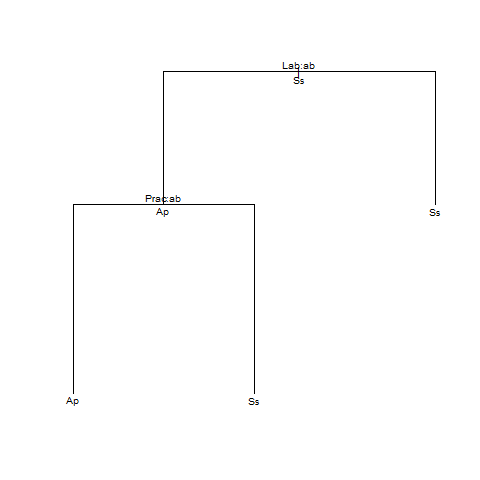
\includegraphics[width=\textwidth]{classT}

%%%%%%%%%%%%%%%%%%%%%%%%%%%%%%%%%%%%%%%%%%%%%%%%%%% 1.2 %%%%%%%%%%%%%%%%%%%%%%%%%%%%%%%%%%%%%%%%%%%%%%%%%%%

\subsection{Análisis de regresión lineal.}
En este caso trabajaremos con datos de planetas, en concreto su Radio y su Diámetro. Los planetas de los que se tienen
los datos son: Mercurio, Venus, Tierra y Marte, y el .txt del que se leen dichos datos tiene el aspecto que
sigue.
\begin{table}[H]
\begin{center}
\begin{tabular}{|c|c|c|}
\hline
Planeta & Radio & Diámetro\\
\hline \hline
Mercurio & 2.4 & 5.4 \\ \hline
Venus & 6.1 & 5.2 \\ \hline
Tierra & 6.4 & 5.5 \\ \hline
Marte & 3.4 & 3.9 \\ \hline
\end{tabular}
\end{center}
\end{table}

\bigskip
Al igual que anteriormente, es necesario leer dicho fichero y pasarlo a dataframe.
\begin{Schunk}
\begin{Sinput}
> planetas<-read.table("./Datos/Planetas.txt")
> muestraP<-data.frame(planetas)
\end{Sinput}
\end{Schunk}

\bigskip
El análisis de regresión se hace mediante el uso de la función \textbf{lm} contenida en el paquete stats. Cabe destacar que el primero
de sus argumentos es de tipo \textit{fórmula} donde una expresión de la forma y \textasciitilde{} model se interpreta como una especificación de que 
la respuesta \texttt{y} está modelada por un predictor lineal especificado simbólicamente por model, es decir, en nuestro caso model=x por lo que
su ejecución queda como:
\begin{Schunk}
\begin{Sinput}
> regresionP<-lm(D~R,data=muestraP)
> regresionP
\end{Sinput}
\begin{Soutput}
Call:
lm(formula = D ~ R, data = muestraP)

Coefficients:
(Intercept)            R  
     4.3624       0.1394  
\end{Soutput}
\end{Schunk}

\bigskip
De acuerdo a la ecuación de una recta \texttt{y=a+b*x}, el primero de los coeficientes es el término independiente (a), y el segundo
de ellos la b.

\bigskip
\begin{Schunk}
\begin{Sinput}
> source("./Funciones/anovaR.R")
> (calcularRecta(planetas$R,planetas$D,mean(planetas$R),mean(planetas$D)))
\end{Sinput}
\begin{Soutput}
[[1]]
[1] 4.149862

[[2]]
[1] 0.1858225
\end{Soutput}
\begin{Sinput}
> (desviacion(planetas$R,mean(planetas$R)))
\end{Sinput}
\begin{Soutput}
[1] 1.715189
\end{Soutput}
\begin{Sinput}
> (cov(planetas$R,planetas$D))
\end{Sinput}
\begin{Soutput}
[1] 0.5466667
\end{Soutput}
\end{Schunk}

\bigskip
Para mostrar el gráfico de dispersión y la recta de ajuste es necesario hacer uso de varias librerías.
\begin{Schunk}
\begin{Sinput}
> library(foreign)
> library(ggplot2)
> library(psych)
\end{Sinput}
\end{Schunk}

\bigskip
Estas librerías se usan en funciones externas usadas para representar los gráficos requeridos. En dicha función es necesario
indicar las columnas de los datos con los que se realizará la regresión.
\begin{Schunk}
\begin{Sinput}
> source("Funciones/plotDisp.R")
> plotDisp(planetas,1,2,regresionP,"Radio","Diametro","regPlanetas.png")
\end{Sinput}
\end{Schunk}
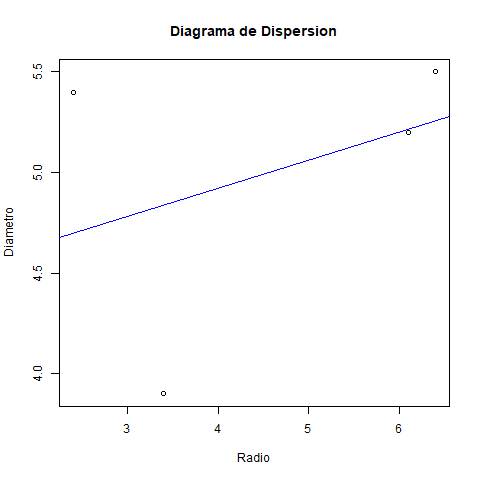
\includegraphics[width=\textwidth]{regPlanetas}

%%%%%%%%%%%%%%%%%%%%%%%%%%%%%%%%%%%%%%%%%%%%%%%%%%% 2.1 %%%%%%%%%%%%%%%%%%%%%%%%%%%%%%%%%%%%%%%%%%%%%%%%%%%

\section{Segunda parte}
\subsection{Función de clasificación.}
En este ejercicio usaremos datos correspondientes a ventas de coches, en concreto son 10 muestras compuestas por: TipoCarnet, 
NúmeroRuedas, NúmeroPasajeros y TipoVehículo.

\bigskip
Para introducir estos datos en el algoritmo a usar es necesario tener un fichero \texttt{.txt} con el
siguiente aspecto.
\begin{table}[H]
\begin{center}
\begin{tabular}{|c|c|c|c|c|}
\hline
Vehículo & TipoCarnet & NúmeroRuedas & NúmeroPasajeros & TipoVehículo\\
\hline \hline
v1 & B & 4 & 5 & Coche \\ \hline
v2 & A & 2 & 2 & Moto \\ \hline
v3 & N & 2 & 1 & Bicicleta \\ \hline
v4 & B & 6 & 4 & Camión \\ \hline
v5 & B & 4 & 6 & Coche \\ \hline
v6 & B & 4 & 4 & Coche \\ \hline
v7 & N & 2 & 2 & Bicicleta \\ \hline
v8 & B & 2 & 1 & Moto \\ \hline
v9 & B & 6 & 2 & Camión \\ \hline
v10 & N & 2 & 1 & Bicicleta \\ \hline
\end{tabular}
\end{center}
\end{table}

\bigskip
Procedemos a leer dicho fichero como anteriormente y pasarlo a dataframe.
\begin{Schunk}
\begin{Sinput}
> vehiculos<-read.table("./Datos/Vehiculos.txt")
> muestraV<-data.frame(vehiculos)
\end{Sinput}
\end{Schunk}

\bigskip
Nuestros datos ya se encuentran preparados para aplicarles la función \textbf{rpart.} La clasificación a obtener será el tipo de
vehículo al que pertenece cada uno de ellos.
\begin{Schunk}
\begin{Sinput}
> clasV<-rpart(TV~.,data=muestraV,method="class",minsplit=1)
> clasV
\end{Sinput}
\begin{Soutput}
n= 10 

node), split, n, loss, yval, (yprob)
      * denotes terminal node

 1) root 10 7 Bicicleta (0.3000000 0.2000000 0.3000000 0.2000000)  
   2) TC=N 3 0 Bicicleta (1.0000000 0.0000000 0.0000000 0.0000000) *
   3) TC=A,B 7 4 Coche (0.0000000 0.2857143 0.4285714 0.2857143)  
     6) NR>=3 5 2 Coche (0.0000000 0.4000000 0.6000000 0.0000000)  
      12) NR>=5 2 0 Camion (0.0000000 1.0000000 0.0000000 0.0000000) *
      13) NR< 5 3 0 Coche (0.0000000 0.0000000 1.0000000 0.0000000) *
     7) NR< 3 2 0 Moto (0.0000000 0.0000000 0.0000000 1.0000000) *
\end{Soutput}
\end{Schunk}

\bigskip
Procedemos a mostrar el árbol de clasificación.
\begin{Schunk}
\begin{Sinput}
> plotTree(clasV, "classTreeV.png")
\end{Sinput}
\end{Schunk}
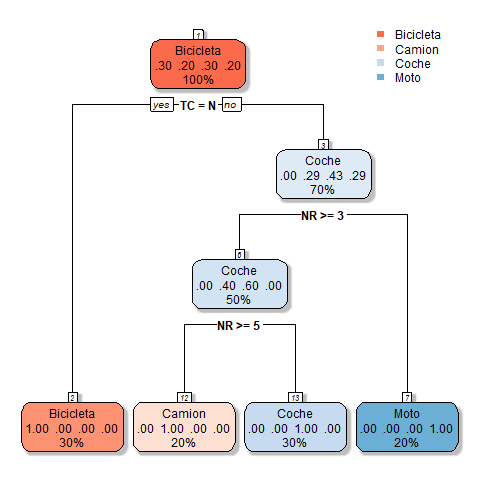
\includegraphics[width=\textwidth]{classTreeV}

\bigskip
Por último, se aplica la función \textbf{tree} a nuestros datos.
\begin{Schunk}
\begin{Sinput}
> classTV<-tree(TV~.,data=muestraV,mincut=1,minsize=2,split="gini")
> classTV
\end{Sinput}
\begin{Soutput}
node), split, n, deviance, yval, (yprob)
      * denotes terminal node

 1) root 10 27.320 Bicicleta ( 0.3000 0.2000 0.3000 0.2000 )  
   2) NP < 1.5 3  3.819 Bicicleta ( 0.6667 0.0000 0.0000 0.3333 )  
     4) TC: B 1  0.000 Moto ( 0.0000 0.0000 0.0000 1.0000 ) *
     5) TC: N 2  0.000 Bicicleta ( 1.0000 0.0000 0.0000 0.0000 ) *
   3) NP > 1.5 7 17.880 Coche ( 0.1429 0.2857 0.4286 0.1429 )  
     6) NP < 3 3  6.592 Bicicleta ( 0.3333 0.3333 0.0000 0.3333 )  
      12) TC: A 1  0.000 Moto ( 0.0000 0.0000 0.0000 1.0000 ) *
      13) TC: B,N 2  2.773 Bicicleta ( 0.5000 0.5000 0.0000 0.0000 )  
        26) TC: B 1  0.000 Camion ( 0.0000 1.0000 0.0000 0.0000 ) *
        27) TC: N 1  0.000 Bicicleta ( 1.0000 0.0000 0.0000 0.0000 ) *
     7) NP > 3 4  4.499 Coche ( 0.0000 0.2500 0.7500 0.0000 )  
      14) NR < 5 3  0.000 Coche ( 0.0000 0.0000 1.0000 0.0000 ) *
      15) NR > 5 1  0.000 Camion ( 0.0000 1.0000 0.0000 0.0000 ) *
\end{Soutput}
\end{Schunk}

\begin{Schunk}
\begin{Sinput}
> plotT(classTV, "classTV.png")
\end{Sinput}
\end{Schunk}
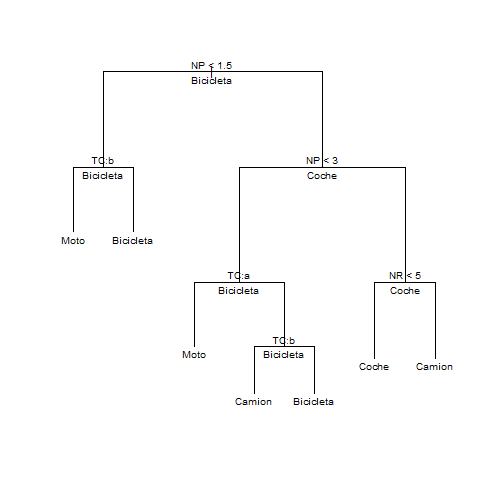
\includegraphics[width=\textwidth]{classTV}

%%%%%%%%%%%%%%%%%%%%%%%%%%%%%%%%%%%%%%%%%%%%%%%%%%% 2.2 %%%%%%%%%%%%%%%%%%%%%%%%%%%%%%%%%%%%%%%%%%%%%%%%%%%
\subsection{Análisis de regresión lineal.}
En este caso tenemos que hacer un análisis de regresión lineal para 4 muestras distintas compuestas
por pares de datos.

\bigskip
Como en ocasiones anteriores, procedemos a leer dichas muestras y pasarlas a dataframe.
\begin{Schunk}
\begin{Sinput}
> pares<-read.table("./Datos/Pares.txt")
> muestraPS<-data.frame(pares)
\end{Sinput}
\end{Schunk}

\bigskip
El análisis de regresión se hace mediante el uso de la función \textbf{lm.} En este caso será neceario hacer cuatro análisis diferentes.
\begin{Schunk}
\begin{Sinput}
> (r1<-lm(V2~V1,data=muestraPS))
\end{Sinput}
\begin{Soutput}
Call:
lm(formula = V2 ~ V1, data = muestraPS)

Coefficients:
(Intercept)           V1  
     3.0001       0.5001  
\end{Soutput}
\begin{Sinput}
> (r2<-lm(V4~V3,data=muestraPS))
\end{Sinput}
\begin{Soutput}
Call:
lm(formula = V4 ~ V3, data = muestraPS)

Coefficients:
(Intercept)           V3  
      3.001        0.500  
\end{Soutput}
\begin{Sinput}
> (r3<-lm(V6~V5,data=muestraPS))
\end{Sinput}
\begin{Soutput}
Call:
lm(formula = V6 ~ V5, data = muestraPS)

Coefficients:
(Intercept)           V5  
     3.0025       0.4997  
\end{Soutput}
\begin{Sinput}
> (r4<-lm(V8~V7,data=muestraPS))
\end{Sinput}
\begin{Soutput}
Call:
lm(formula = V8 ~ V7, data = muestraPS)

Coefficients:
(Intercept)           V7  
     3.0017       0.4999  
\end{Soutput}
\end{Schunk}

\bigskip
De acuerdo a la ecuación de una recta \texttt{y=a+b*x}, el primero de los coeficientes es el término independiente (a), y el segundo
de ellos la b.

\bigskip
Mostraremos estos análisis en una misma figura mediante el uso de:
\begin{Schunk}
\begin{Sinput}
> source("Funciones/plotDisp2.R")
> plotDisp2
\end{Sinput}
\begin{Soutput}
function(data, r1, r2, r3, r4, ruta) {

    png(paste("./tmp/",ruta,sep=""))

    par(mfrow = c(2, 2))

    plot(data[,1], data[,2], xlab="x", ylab="y", main="Muestra 1")
    abline(r1, col = "red")

    plot(data[,3], data[,4], xlab="x", ylab="y", main="Muestra 2")
    abline(r2, col = "blue")

    plot(data[,5], data[,6], xlab="x", ylab="y", main="Muestra 3")
    abline(r3, col = "green")

    plot(data[,7], data[,8], xlab="x", ylab="y", main="Muestra 4")
    abline(r4, col = "yellow")

    dev.off()
}
\end{Soutput}
\end{Schunk}

\bigskip
Procedemos a su ejecución.
\begin{Schunk}
\begin{Sinput}
> plotDisp2(pares, r1, r2, r3, r4, "rPares.png")
\end{Sinput}
\end{Schunk}
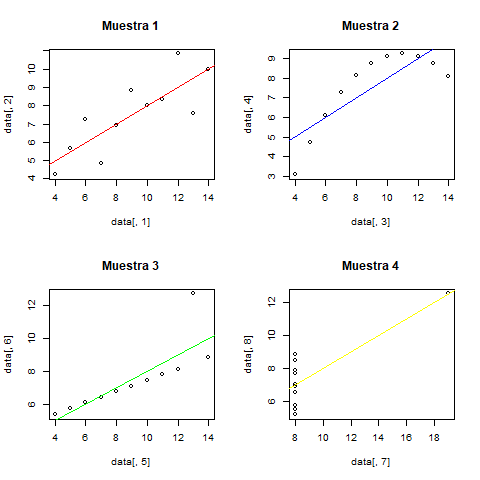
\includegraphics[width=\textwidth]{rPares}

%%%%%%%%%%%%%%%%%%%%%%%%%%%%%%%%%%%%%%%%%%%%%%%%%%% 2.3 %%%%%%%%%%%%%%%%%%%%%%%%%%%%%%%%%%%%%%%%%%%%%%%%%%%
\subsection{Desarrollo por parte del alumno.}

\bigskip
Para la parte de \textbf{clasificación} usaremos datos de \textit{Setas}, las cuales clasificaremos en función de si son venenosas (p) o 
comestibles (e), es decir, los tipos de setas que encontramos en el archivo. Procedemos a leer dicho fichero como en prácticas anteriores
haciendo uso de la librería readr.
\begin{Schunk}
\begin{Sinput}
> install.packages("readr")
> library("readr")
> setas<-read.csv("./Datos/mushrooms.csv")
\end{Sinput}
\end{Schunk}

\bigskip
Los atributos que encontramos en este documento son:
\begin{itemize}
\item class: edible=e, poisonous=p
\item cap-shape: bell=b,conical=c,convex=x,flat=f, knobbed=k,sunken=s
\item cap-surface: fibrous=f,grooves=g,scaly=y,smooth=s
\item cap-color: brown=n,buff=b,cinnamon=c,gray=g,green=r,pink=p,purple=u,red=e,\\white=w,yellow=y
\item bruises: bruises=t,no=f
\item odor: almond=a,anise=l,creosote=c,fishy=y,foul=f,musty=m,none=n,pungent=p,spicy=s
\item gill-attachment: attached=a,descending=d,free=f,notched=n
\item gill-spacing: close=c,crowded=w,distant=d
\item gill-size: broad=b,narrow=n
\item gill-color: black=k,brown=n,buff=b,chocolate=h,gray=g, green=r,orange=o,pink=p,\\purple=u,red=e,white=w,yellow=y
\item stalk-shape: enlarging=e,tapering=t
\item stalk-root: bulbous=b,club=c,cup=u,equal=e,rhizomorphs=z,rooted=r,missing=?
\item stalk-surface-above-ring: fibrous=f,scaly=y,silky=k,smooth=s
\item stalk-surface-below-ring: fibrous=f,scaly=y,silky=k,smooth=s
\item stalk-color-above-ring: brown=n,buff=b,cinnamon=c,gray=g,orange=o,pink=p,red=e,\\white=w,yellow=y
\item stalk-color-below-ring: brown=n,buff=b,cinnamon=c,gray=g,orange=o,pink=p,red=e,\\white=w,yellow=y
\item veil-type: partial=p,universal=u
\item veil-color: brown=n,orange=o,white=w,yellow=y
\item ring-number: none=n,one=o,two=t
\item ring-type: cobwebby=c,evanescent=e,flaring=f,large=l,none=n,pendant=p,sheathing=s,zone=z
\item spore-print-color: black=k,brown=n,buff=b,chocolate=h,green=r,orange=o,purple=u,\\white=w,yellow=y
\item population: abundant=a,clustered=c,numerous=n,scattered=s,several=v,solitary=y
\item habitat: grasses=g,leaves=l,meadows=m,paths=p,urban=u,waste=w,woods=d
\end{itemize}

\bigskip
\begin{Schunk}
\begin{Sinput}
> clasM<-rpart(class~.,data=setas,method="class")
> clasM
\end{Sinput}
\begin{Soutput}
n= 8124 

node), split, n, loss, yval, (yprob)
      * denotes terminal node

1) root 8124 3916 e (0.51797144 0.48202856)  
  2) odor=a,l,n 4328  120 e (0.97227357 0.02772643)  
    4) spore.print.color=b,h,k,n,o,u,w,y 4256   48 e (0.98872180 0.01127820) *
    5) spore.print.color=r 72    0 p (0.00000000 1.00000000) *
  3) odor=c,f,m,p,s,y 3796    0 p (0.00000000 1.00000000) *
\end{Soutput}
\end{Schunk}

\bigskip
Procedemos a mostrar el árbol de clasificación.
\begin{Schunk}
\begin{Sinput}
> plotTree(clasM, "classTreeM.png")
\end{Sinput}
\end{Schunk}
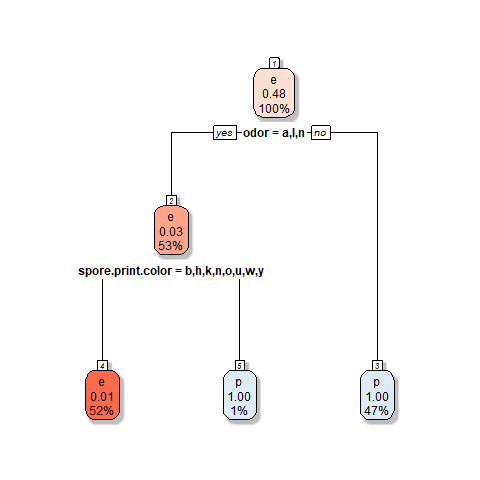
\includegraphics[width=\textwidth]{classTreeM}

\bigskip
Función de clasificación obtenida:
\begin{itemize}
\item Si el olor no es anisado ni almendrado, se trata de una seta venenosa.
\item En caso contrario, si su color no es verde, estamos ante una seta comestible, para el resto es venenosa.
\end{itemize}

\bigskip
Para usar la función \texttt{predict} con el fin de generar predicciones a partir de un modelo entrenado, necesitamos
un set de entrenamiento y otro de prueba que compruebe la eficacia de las predicciones. Para obtener estos sets utilizamos
la función \texttt{sample\_frac} la cual pertenece al paquete \textbf{dplyr}, además por el parámetro \textit{newdata} es
necesario el uso del paquete \textbf{e1071.} Posteriormente, con la función \texttt{confusionMatrix} obtenemos la matriz de
confusión del conjunto de pruebas, dicha función se encuentra en el paquete \textbf{caret}.

\bigskip
Instalación de paquetes.
\begin{Schunk}
\begin{Sinput}
> install.packages("dplyr")
> library("dplyr")
> install.packages("e1071")
> library("e1071")
> install.packages("caret")
> library("caret")
\end{Sinput}
\end{Schunk}

\bigskip
Separación de los datos para el set de entrenamiento y pruebas.
\begin{Schunk}
\begin{Sinput}
> setasTrain<-sample_frac(setas,.7)
> setasP<-setdiff(setas,setasTrain)
\end{Sinput}
\end{Schunk}

\bigskip
Mostramos la función de clasificación perteneciente al 70\% del conjunto de datos.
\begin{Schunk}
\begin{Sinput}
> clas70<-rpart(class~.,data=setasTrain,method="class")
> plotTree(clas70, "classTree70.png")
\end{Sinput}
\end{Schunk}
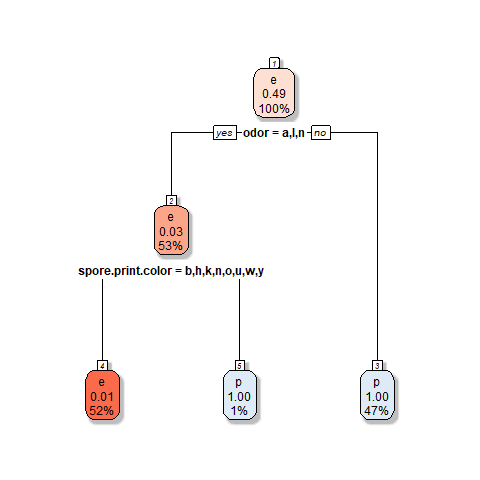
\includegraphics[width=\textwidth]{classTree70}

\bigskip
Ejecución de la predicción y la posterior matriz de confusión.
\begin{Schunk}
\begin{Sinput}
> prediccion<-predict(clas70, newdata=setasP, type="class")
> cm<-confusionMatrix(prediccion, setasP[["class"]])
\end{Sinput}
\end{Schunk}

\bigskip
Una vez calculada la matriz de confusión procedemos a mostrarla gráficamente.
\begin{Schunk}
\begin{Sinput}
> source("./Funciones/drawCM.R")
> drawCM(cm,"cmSetas.png")
\end{Sinput}
\end{Schunk}
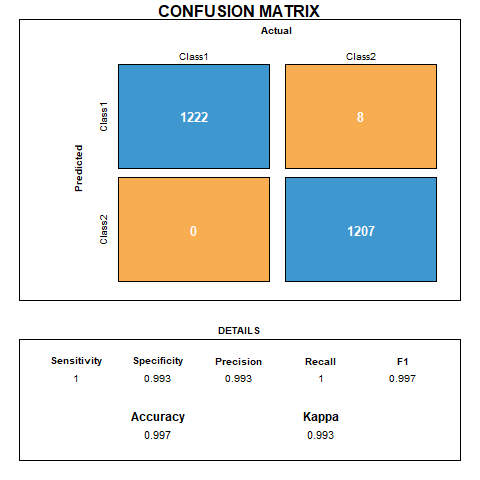
\includegraphics[width=\textwidth]{cmSetas}

\bigskip
En la parte del \textbf{análisis de regresión lineal} usaremos datos pertenecientes al clima, de los cuales usaremos la 
temperatura y humedad.

\bigskip
En primer lugar debemos leer estos datos contenidos en un .csv y convertirlos en dataframe.
\begin{Schunk}
\begin{Sinput}
> w<-read.csv("./Datos/weather.csv")
> weather<-data.frame(w)
\end{Sinput}
\end{Schunk}

\bigskip
Guardamos en dos variables los datos de temperatura y humedad para facilitar su utilización.
\begin{Schunk}
\begin{Sinput}
> t<-weather$tempm
> h<-weather$hum
\end{Sinput}
\end{Schunk}

\bigskip
De estos valores obtenemos tanto la \textbf{Covarianza} como la \textbf{Correlación.}
\begin{Schunk}
\begin{Sinput}
> (cov(h,t))
\end{Sinput}
\begin{Soutput}
[1] -71.96809
\end{Soutput}
\begin{Sinput}
> (cor(h,t))
\end{Sinput}
\begin{Soutput}
[1] -0.9778414
\end{Soutput}
\end{Schunk}

\bigskip
El análisis de la covarianza resulta muy complicado ya que se trata de una medida que depende mucho del dominio de los datos
a estudiar, es decir, no se encuentra normalizada. Por ello surge la correlación, una medida cuyo valor se encuentra en el
intervalo [-1,1]. Un valor de la correlación igual a -1 (recta con pendiente negativa) o 1 (recta con pendiente positiva), indicará
un buen ajuste de los datos a la recta de regresión.

\bigskip
Realización del análisis de regresión.
\begin{Schunk}
\begin{Sinput}
> (regresionW<-lm(t~h,data=weather))
\end{Sinput}
\begin{Soutput}
Call:
lm(formula = t ~ h, data = weather)

Coefficients:
(Intercept)            h  
     37.398       -0.291  
\end{Soutput}
\end{Schunk}
\bigskip
De acuerdo a la ecuación de una recta \texttt{y=a+b*x}, el primero de los coeficientes es el término independiente (a), y el segundo
de ellos la b.

\bigskip
Mostrar gráficamente la recta de regresión.
\begin{Schunk}
\begin{Sinput}
> plotDisp(weather,7,12,regresionW,"Humedad","Temperatura","regWeather.png")
\end{Sinput}
\end{Schunk}
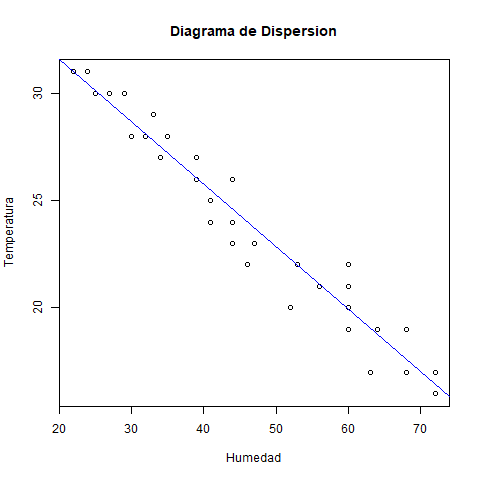
\includegraphics[width=\textwidth]{regWeather}

\end{document}
